\chapter{Application development}
Based on the theoretical notions described above, we implemented the basics of a facial authentication system that would get real-time feed from the laptop's webcam, detect if there is a face in front of it and upon confirming it is a live one and not a spoof attack, it would search for a face in it's database that is sufficiently similar and assign it's known identity to the face in front of the camera.	

\section{Implementation language}
We chose Python as the main code language for multiple reasons ranging from the strong support it has from the opensource community, which put at our disposal great implementations of the tools we needed to create the system we started out with in mind to the well fitting of this language with our pragmatic approach.
\section{Used frameworks}
Having as target the creation of a reliable system, we favored only the most solid frameworks that could be found. This guided us in using Scikit-learn \cite{scikit-learn} in anything related to data analysis as classifiers, metrics or preprocessing methods; this framework being supported, among others, by Google and INRIA(French Institute for Reasearch in Computer Science and Automation). In matters of image processing from reading an image, getting video feed from webcam to changing the colorspace of an image and applying afine transformations we used OpenCV \cite{opencv_library} as it was designed for computational efficiency with a focus on real-time applications. We also used Scykit-image \cite{scikit-image} for it's implementation of the local binary patterns descriptor. For one of the most important parts of the system, the CNN used for image embedding, we used the OpenFace \cite{amos2016openface} implementation of the FaceNet \cite{SchroffKP15} system.
\section{Application architecture}
\begin{figure}[H]
	\captionsetup{width=15cm,font=small}
	\begin{center}
		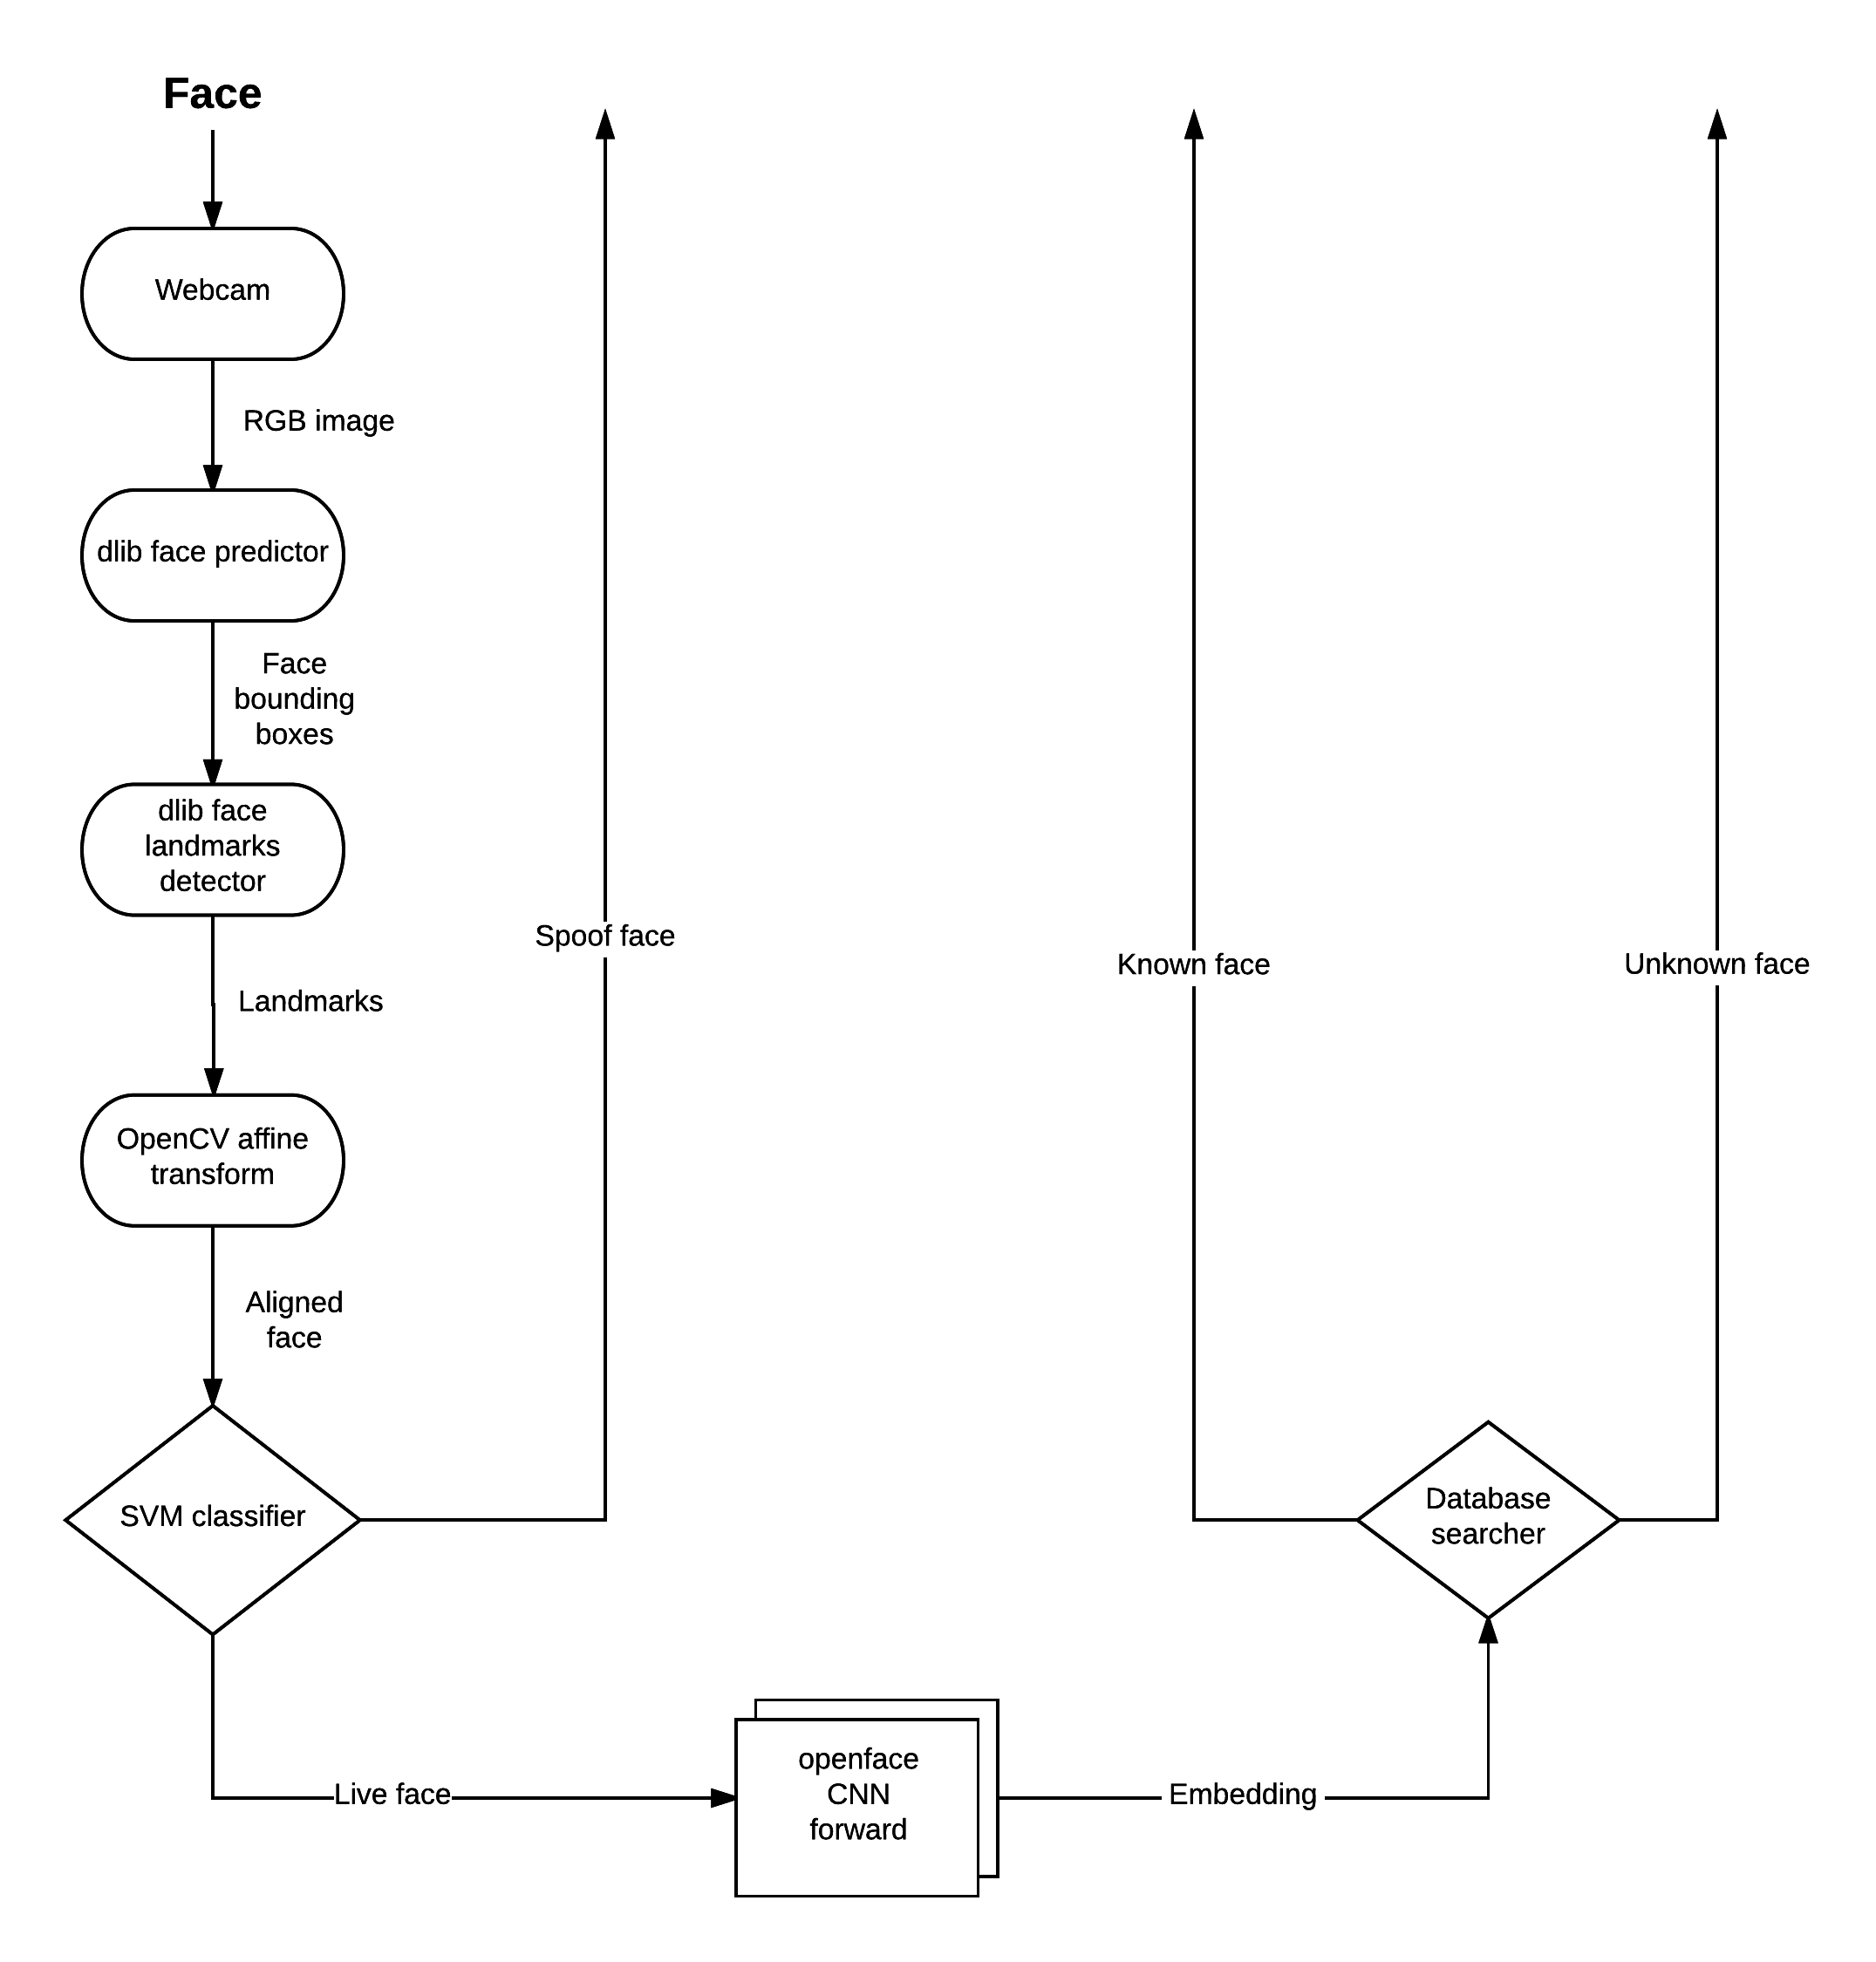
\includegraphics[width=15cm,height=10cm]{application_architecture}
	\end{center}
	\caption[Application architecure]{Visual representation of the components of the application}
	\label{fig:application_architecture}
\end{figure}
The application was designed so that it would have a component for each theoretical aspect described above. Therefore, in the application, the stages from reading an image to asigning and identity to a face are as follows: firstly, a frame is captured using the webcam of the laptop or an external one with the help of opencv framework, then the dlib \cite{dlib09} face predictor is used to determine all face bounding boxes in the image. 
Each bounding box is then used to crop the face from the full image and, upon that, the dlib facial landmark detector is aplied to it, which computes the 68 dimmensional array with points corresponding to each landmark. 
Then the opencv implementation of affine transformation is used to align the outer eyes and nose. Having the aligned image of the face, a face spoof validator is used to determine the liveness of it. 
In order to do so, the described sliding windows method was implemented where for each window three LBPs with parameters $(P,R) \in \{(8,1), (8,2), (16,2)\}$ are employed using the LBP implementation available in the \textit{feature} module of the skimage \cite{scikit-image} framework for which we set the method to "nri\_uniform" representing the non-rotation invariant version\textbf{Here it should be defined the rotation and nonrotation invariant versions of lbp} of the uniform local binary pattern. A thing to note here is that, even though in the literature the uniform LBP is nonrotation invariante, in the scikit-image \cite{scikit-image} implementation, setting the method to simply uniform results in the computation of a rotation invariant descriptor. 
\begin{figure}[H]
	\captionsetup{width=15cm,font=small}
	\begin{center}
		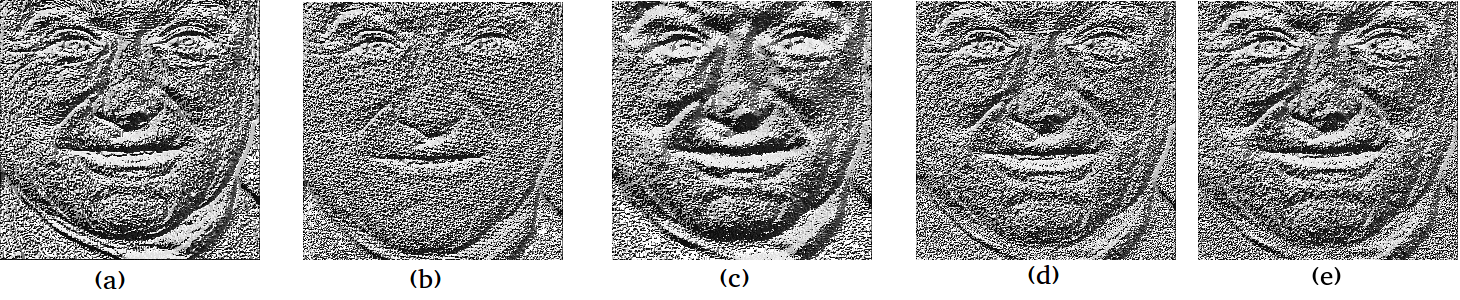
\includegraphics[width=15cm,height=4cm]{visual_results_lbp}
	\end{center}
	\caption[LBP feature visualisation on faces]{Here we present the visualisation of the basic LBP with parameters $(P,R) = (8,1)$ for: (a) real image, (b) nexus 5 spoof medium taken with rear camera of a nexus 5, (c) nexus 5 spoof medium taken with front camera of a nexus 5, (d) printed photo spoof medium taken with rear camera of a nexus 5 and (e) printed photo spoof medium taken with front camera of a nexus 5}
	\label{fig:application_architecture}
\end{figure}
Once the descriptor is computed, a previously trained SVM with linear kernel is then used to predict the probability of liveness. \begin{figure}[H]
	\captionsetup{width=15cm,font=small}
	\begin{center}
		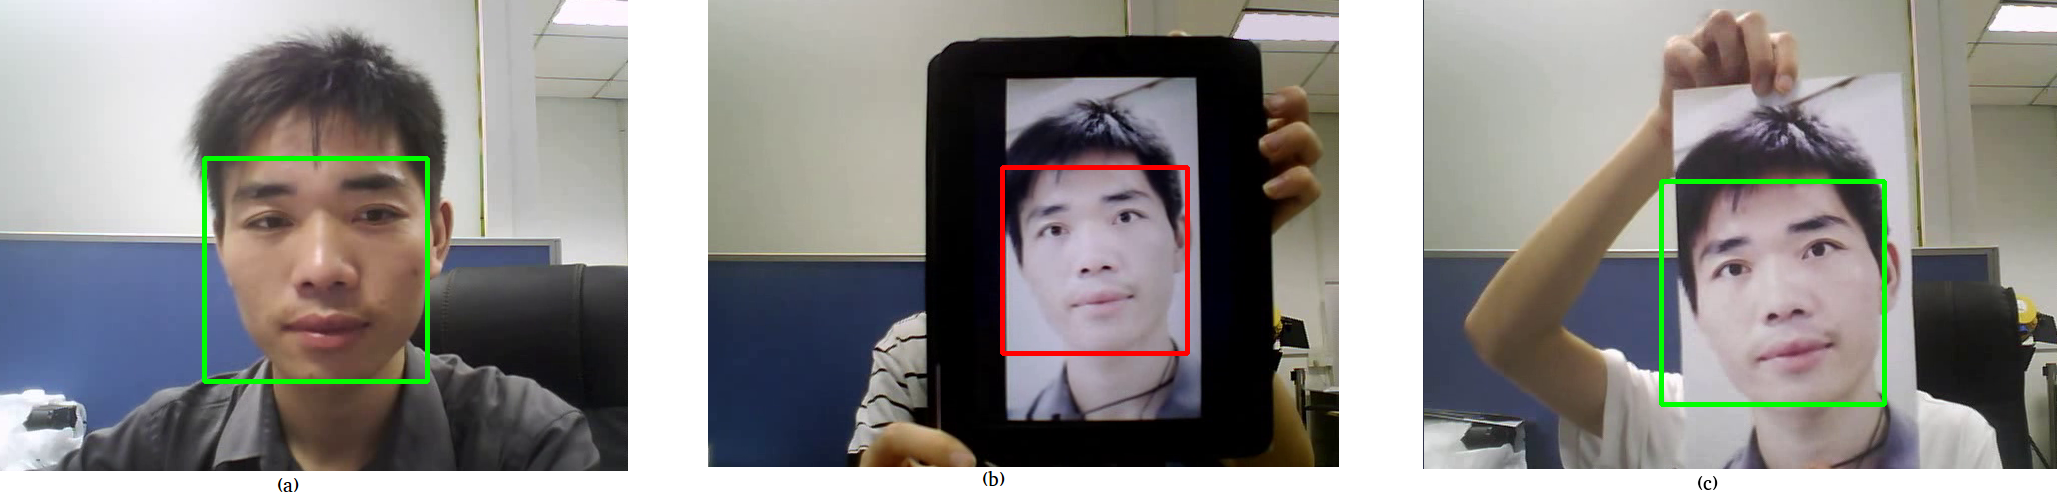
\includegraphics[width=15cm,height=4cm]{spoof_classification_results}
	\end{center}
	\caption[Results on spoof classification]{Here we present the results of the SVM trained on the CASIA database for an example in the test data: (a) is the live face which is correctly classified as being valid, (b) is a spoof face on an IPAD which is correctly classified as being invalid and (c) is a spoof face on a printed paper which is misclassified as being valid}
	\label{fig:spoof_classification_results}
\end{figure} A threshold of 0.5 is used to map the probabilities in two classes. If the face is not valid, the opencv rectangle drawing functionality is used to put a red bounding box over the spoof face. In the other case, we forward the face through the openface neural network obtaining the 128 dimensional mapping of it. We then iterate through the database of known faces and find the face whose representation is closest to the previously computed one. If this minimum distance is smaller than the threshold used for identity matching, we put a green bounding box around the face \textbf{PUT HERE A FIGURE WITH A RECOGNIZED FACE AND ONE NOT} and append the name corresponding to the matched face. 
\section{Running time}
